
\documentclass{report}

\usepackage{lmodern}
\usepackage[T1]{fontenc}
\usepackage[utf8]{inputenc}
\usepackage{mathtools}
\usepackage{graphicx}
\usepackage{sectsty} % Para cambiar el tamanio de los titulos
\usepackage[lmargin=1in, rmargin=0.75in]{geometry}

\setcounter{section}{-1}
\sectionfont{\LARGE}
\newcommand\tab[1][0.6cm]{\hspace*{#1}}
\newcommand\nl{\newline\tab}
\renewcommand\labelenumii{\theenumi.\arabic{enumii}.}
\renewcommand\thesection{\arabic{section}.} %Para que las secciones no se nombren como chapter.section (0.1, 0.2 etc)
\renewcommand\labelitemi{$\cdot$ }

\title{Practica 4 Arquitectura de Ordenadores}
\author{Lucía Asencio y Juan Riera}
\date{Diciembre 2017}

%No sé si esto es útil ahora, pero probablemente lo será algún día
%Es para introducir código en documentos!!
\usepackage{listings}
\usepackage{color}

\definecolor{dkgreen}{rgb}{0,0.6,0}
\definecolor{gray}{rgb}{0.5,0.5,0.5}
\definecolor{mauve}{rgb}{0.58,0,0.82}

\lstset{frame=tb,
	language=Java,
	aboveskip=3mm,
	belowskip=3mm,
	showstringspaces=false,
	columns=flexible,
	basicstyle={\small\ttfamily},
	numbers=none,
	numberstyle=\tiny\color{gray},
	keywordstyle=\color{blue},
	commentstyle=\color{dkgreen},
	stringstyle=\color{mauve},
	breaklines=true,
	breakatwhitespace=true,
	tabsize=3
}
%Hasta aqui la cosa rara de añadir codigo



\begin{document}
	\maketitle
	
	\section{Información sobre la topología del sistema}
	
	\tab Con el comando \texttt{cpuinfo} pudimos comprobar que, en los ordenadores del laboratorio, disponemos de 4 cpu\_cores y 4 siblings (4 reales y 4 virtuales). A partir de aquí, sabemos que, en caso de existir \textit{hyperthreading}, este no está habilitado. 
	\nl Para comprobar si existía, buscamos en internet y comprobamos que el procesador no disponía de \textit{hyperthreading}.
	\nl  De los 4 cores reales, 3 son de 800MHz y 1 de 1000MHz
	
	\newpage
	\section{Programas básicos de OpenMP}
	
	\begin{center}
		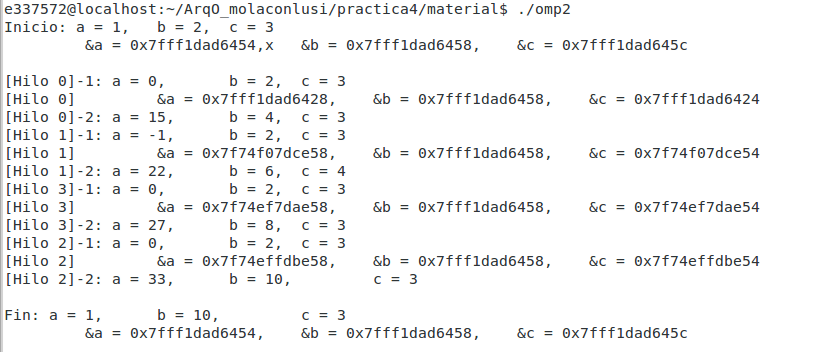
\includegraphics[width=6in]{imagenes_memoria/ej2.png}
	\end{center}
	
	\begin{enumerate}
		\item{\textbf{\tab ¿Se	pueden	lanzar	más	threads	que	cores	tenga	el	sistema?¿Tiene	sentido	hacerlo?}	\nl El programa nos permite lanzar tantos hilos como queramos dentro de cierto margen (32037 es el máximo que nos ha permitido lanzar), pero como no disponemos de \textit{hyperthreading}, no tendría sentido hacerlo ya que cada core no permitiría la ejecución de más de un thread a la vez.}
		\item{\textbf { \tab ¿Cuántos	threads	debería	utilizar	en	los	ordenadores	del	laboratorio?	¿y	en	su	propio	equipo?	} \nl 
			A la vista de la salida de \texttt{cpuinfo}, sabemos que el número idóneo de hilos es 4.\nl No disponemos de un ordenador personal.}
		\item{\textbf {\tab ¿Cómo se comporta OpenMP	cuando	declaramos	una	variable	privada?		} \nl Las variables privadas declaradas como "private" apuntarán a una dirección de memoria cualquiera que tendrá valores residuales. Por otro lado si están declaradas como \texttt{firstprivate} tendrán el valor de incialización de la variable con el mismo nombre presente fuera de los threads. }
		\item{\textbf {\tab ¿Qué ocurre	con	el valor de una variable privada al comenzar a	ejecutarse	la región paralela? } \nl Las variables delcadaras con \texttt{private} se deben inicializar en cada hilo, si no, ocurrirá como ocurre en la ejecución del programa, que tendrán valores indeterminados. En este caso tienen 0 o -1 porque apuntan a direcciones que contienen todo 0's o todo F's. Si se declara con \texttt{firstprivate} no hay este problema, ya que la variable queda con el valor de inicialización original.}
		\item{\textbf {\tab ¿Qué	ocurre	con	el	valor	de	una	variable	privada	al	finalizar	la	región	paralela?		} \nl Como observamos, las direcciones de memoria de las variables privadas son distintas de las de las originales, tanto en el caso de las declaradas con "private" como en el de las declaradas con \texttt{firstprivate}. Por ello, su valor se pierde al terminar la ejecucion del thread.}
		\item{\textbf {\tab ¿Ocurre	lo	mismo	con	las	variables	públicas?		} \nl 
			En el caso de las variables públicas, sus direcciones de memoria son las mismas que las de las variables originales. Por esa razón cuando se editan en lo threads se edita la variable original, y por tanto cuando acaban los threads se mantiene el valor.}
		
	\end{enumerate}
	
	\newpage
	\section {Paralelizar el producto escalar}
	\begin{enumerate}
		\item{\textbf{\tab ¿En	qué	caso	es	correcto	el	resultado?	}\nl De las ejecuciones paralelas, el resultado sólo es correcto en la ejecución \texttt{par2}.
		}
		\item{\textbf{\tab ¿A	qué	se	debe	esta	diferencia?	}\nl
			Como en par1 la variable sum es pública, no se controla la concurrencia de operaciones sobre ella  y pueden ocurrir distintos sucesos que den lugar a un error en el resultado. Por ejemplo: que el thread 1 coja el valor de sum, el thread 2 coge el mismo valor sum, ejecuta su operación y lo guarda, y al final el thread 1 ejecuta su operación con el valor antiguo de sum, guardando un valor erróneo en la variable. Sin embargo, con el uso de reduction, la segunda versión si controla el acceso a esta variable: cada hilo hace su propia suma y luego se suman todos los resultados. 
		}
		\textit{\nl \newline \textbf{Nota:} el enunciado indicaba que teníamos que usar vectores que tardaran em multiplicarse hasta 10 segundos. Las gráficas obtenidas no van a representar estos tiempos por lo siguiente: aunque la salida del programa nos daba tiempos de ejecución de apenas 2 segundos, añadiendo otro timeval para saber el tiempo total de ejecución, obteníamos ejecuciones de 20 segundos. Por tanto, aunque en la gráfica se reflejen tiempos bajos, los tiempos reales eran los que la práctica requería.}
		
		\begin{center}
			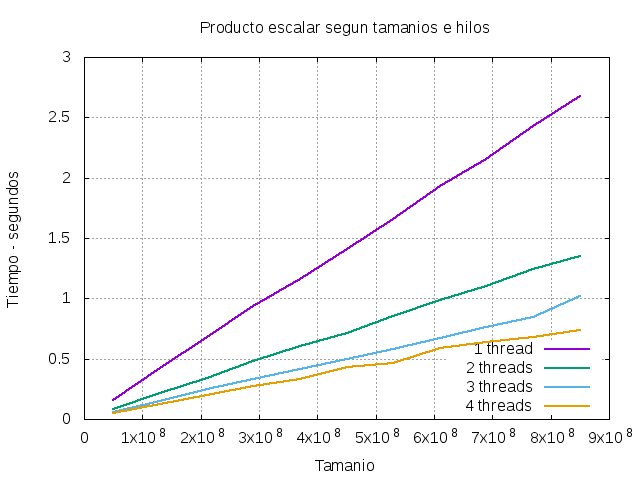
\includegraphics[width=6in]{imagenes_memoria/pescalar.png}
		\end{center}
		\begin{center}
			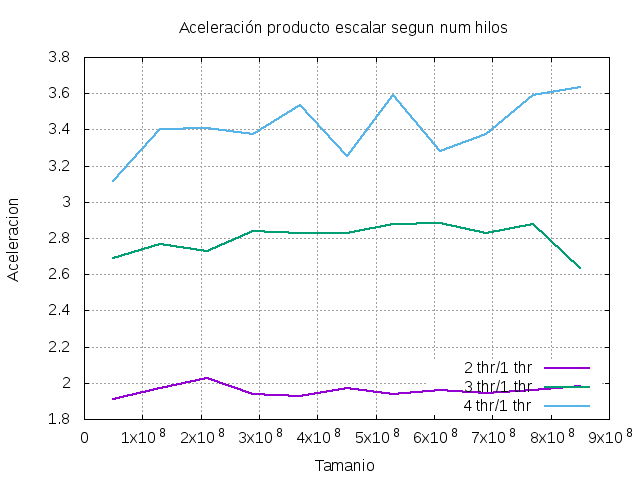
\includegraphics[width=6in]{imagenes_memoria/acc.png}
		\end{center}
		
		\item{\textbf{\tab En	términos	del	tamaño	de	los	vectores,	¿compensa	siempre	lanzar	hilos	para	realizar	el	trabajo	en	
				paralelo,	o	hay	casos	en	los	que	no?	 }\nl
			Como puede deducirse de la primera gráfica, lanzar más hilos ha aumentado en todo caso la eficiencia del programa, y el único caso en que podemos encontrar alguna pega es para el lanzamiento de 4 hilos, que discutimos en la siguiente pregunta. 
			\nl Para 2 hilos, el programa se ejecuta exactamente 2 veces más rápido (véase la gráfica de la aceleración), y para 3 hilos también trabajaba alrededor de 3 veces más rápido que el programa en serie.
		}
		\item{\textbf{\tab Si	compensara	siempre,	¿en	qué	casos	no	compensa	y	por	qué?	}\nl
			A pesar de que trabajar con 4 hilos sea más rápido que trabajar con 3, hemos encontrado una pequeña pega: esperaríamos que el rendimiento con fuera cuatro veces mayor que el del programa de producto escalar en serie, pero no es así. La aceleración medida ronda el 3,5, en lugar de la ideal, que sería 4.
			\nl Esto podría deberse a que el tiempo de inicialización y sincronización de hilos fuera demasiado alto como para conseguir el rendimiento óptimo del programa.
		}
		\item{\textbf{\tab ¿Se	mejora	siempre	el	rendimiento	al	aumentar	el	número	de	hilos	a	trabajar?	Si	no	fuera	así,	¿a	qué	debe	este	efecto?
			}\nl
			Para el número de hilos representados en las gráficas, la respuesta es sí, aunque no siempre tanto como sería deseable (caso de 4 hilos). Sin embargo, sabemos que si seguimos aumentando el número de hilos hasta superar el de los hilos virtuales que soporta el peocesador, no conseguiríamos un rendimiento mayor.
		}
		\item{\textbf{\tab Valore	si	existe	algún	tamaño	del	vector	a	partir	del	cual	el	comportamiento	de	la	aceleración	va	a	
				ser	muy	diferente	del	obtenido	en	la	gráfica.	}\nl
			
		}
	\end{enumerate}
	\newpage
	
	
	\section {Paralelizar la multiplicación de matrices}
	\begin{enumerate}
		\item{\textbf{\tab ¿Cuál	de	las	tres	versiones	obtiene	peor	rendimiento?	¿A	qué	se	debe?}\nl
			La versión que ha obtenido peor rendimiento ha sido la de paralelización del bucle  con un único hilo. La razón de esto se halla en el hecho de que, por un lado, un hilo es el menor nivel de paralelización posible, por otro lado, el número de operaciones paralelizadas no es el suficiente para que salga rentable dicha paralelización en términos de eficiencia, y esto se ve potenciado por el hecho de que la paralelizacion se ejecuta en cada iteración del bucle superior.}
		
		\item{\textbf{\tab ¿Cuál	de	las	tres	versiones	obtiene	mejor	rendimiento?	¿A	qué	se	debe?}\nl
			Tiene mejor rendimiento la version en la que se paraleliza el bucle 3, es decir, el bucle exterior, con 4 hilos. Esto tiene sentido, ya que a más hilos, mientras el número de éstos no supere el número de cores de la máquina, mayor es la paralelización, y mayor es, por tanto, el rendimiento. En cuanto a que el bucle que tiene más sentido paralelizar sea el exterior se debe a que esta es la manera de paralelizar más operaciones. Por ejemplo, el bucle interior ejecuta menos operaciones por cada iteración que cualquiera de los otros.}
		
	\end{enumerate}
	\newpage
	\section{Ejemplo de integración numérica \newline Perdida de rendimiento por el efecto de falso compartir (False
		sharing) en OpenMP}
	\begin{enumerate}
		\item {\textbf{\tab ¿Cuántos rectángulos se utilizan en la versión del programa que se da para realizar la integración numérica?}\nl
			La partición es de $ n=10^8 $ rectángulos.
		}
		\item {\textbf{\tab ¿Qué diferencias observa entre estas dos versiones?}\nl
			En el caso de \texttt{pi\_par1.c}, a cada hilo se le asocian ciertas $h$ de la partición y un elemento de un array compartido. Para cada una de sus $h$, el hilo suma cierto valor a su correspondiente elemento del array.\nl
			En cambio, en \texttt{pi\_par4.c}, cada hilo realiza su propia suma sobre una variable invisible a los demás hilos, y sólo cuando ha completado todos los cálculos que se le habían asignado escribe ese valor en el elemento del array que le corresponde. 
		}
		\item {\textbf{\tab Ejecute las dos versiones recién mencionadas. ¿Se observan diferencias en el resultado obtenido? ¿Y en el rendimiento? Si la respuesta fuera afirmativa, ¿sabría justificar a qué se debe este efecto?}\nl
			A pesar de que en ambos programas la salida indica \texttt{resultado $\pi$: 3.141593}, el rendimiento es muy distinto. En \texttt{./pi\_par4 } tenemos tiempo 0.121272 y en \texttt{./pi\_par1} obtenemos  0.370529, que resulta tres veces más lento.\nl
			La razón es que, en \texttt{pi\_par1.c}, por cada iteración del bucle los hilos actualizan diferentes posiciones del mismo array. Como cada procesador tiene su propia caché donde reside una copia del array, cada actualización de cualquier elemento del mismo debe propagarse hacia arriba, y luego llegar a las cachés distintos procesadores. En cambio, \texttt{pi\_par4.c} sólo escribe en el array una vez por cada hilo (en lugar de una vez por cada hilo e iteración), por lo cual la actualización del mismo no supone un problema en el rendimiento del programa.
		}
		\item {\textbf{\tab Ejecute las versiones paralelas 2 y 3 del programa. ¿Qué ocurre con el resultado y el rendimiento obtenido? ¿Ha ocurrido lo que se esperaba?}\nl
		}
		\item {\textbf{\tab Abra el fichero pi\_par3.c y modifique la línea 32 del fichero para que tome los valores fijos 1, 2, 4, 6, 7, 8, 9, 10 y 12. Ejecute este programa para cada uno de estos valores. ¿Qué ocurre con el rendimiento que se observa?}\nl
		}
		
		
	\end{enumerate}
	
	
\end{document}